\begin{frame}{Real Distributions Are Clustered}
  \begin{columns}[T,onlytextwidth]
    \column{0.48\textwidth}
    \textbf{Goswami's bound makes no assumptions about $S$} --- it holds
    for \emph{every} $S \subseteq [0, 2^L)$.
    \vspace{0.6em}

    \textbf{But real LSM keys are not arbitrary.}
    They concentrate in \emph{dense clusters} separated by \emph{sparse gaps}:
    \begin{itemize}\setlength{\itemsep}{0.15em}
      \item file paths with shared directory prefixes
      \item URLs with shared domain prefixes
      \item consecutive timestamps
      \item geospatial S2 cell IDs
      \item auto-incrementing primary keys
    \end{itemize}
    \vspace{0.6em}

    \column{0.48\textwidth}
    \centering
    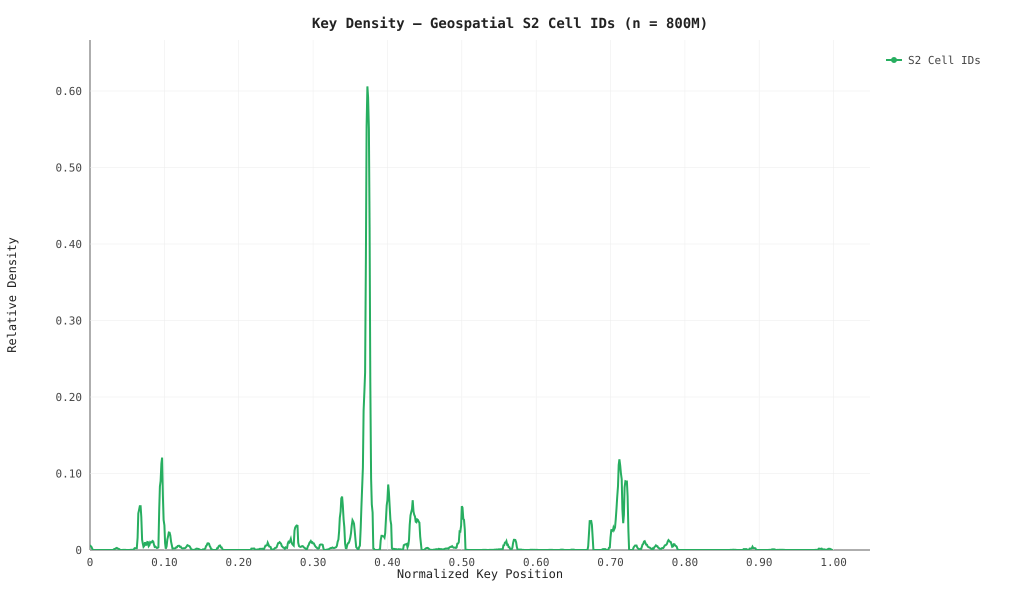
\includegraphics[width=\linewidth, keepaspectratio]{figures/hist_sosd_osm_smoothed}

    \vspace{-0.2em}
    {\footnotesize $n = 8 \cdot 10^8$ S2 cell IDs from SOSD dataset: density is far
    from uniform --- clusters of populated cells alternate with sparse regions.}
  \end{columns}

  \vspace{0.6em}
  \begin{center}
    \textit{Goswami-tight for arbitrary $S$ --- but real $S$ leaves room to compress.}
  \end{center}
\end{frame}
